\section{Генетический триггер Жакоба-Моно}

Рассмотрим модель биохимической регуляции белкового синтеза, предложенную 
Жакобом и Моно в 1964 году и математически разработанную Д.С. Чернавским 
в 1967 году. Эта модель показывает принципиальные возможности триггерных 
систем.

Схема взаимной регуляции двух систем синтеза ферментов (рис. 1). 
Ген-регулятор каждой системы синтезирует неактивный репрессор. 
Этот репрессор, соединяясь с продуктом противоположной системы, образует 
активный комплекс, который реагируя с участком структурного гена, 
называемый опероном, блокирует синтез m-РНК. Таким образом, продукт первой 
системы \( P_1 \) является корепрессором второй системы, а продукт 
второй системы \( P_2 \) -- корепрессором перой. При этом в процессе 
корепрессии могут принимать участие одна, две и более молекул продукта.

\section{Синтез фермента E и катализируемого продукта P}

\begin{wrapfigure}[9]{l}{0.5\textwidth}
    \vspace{-2ex}
    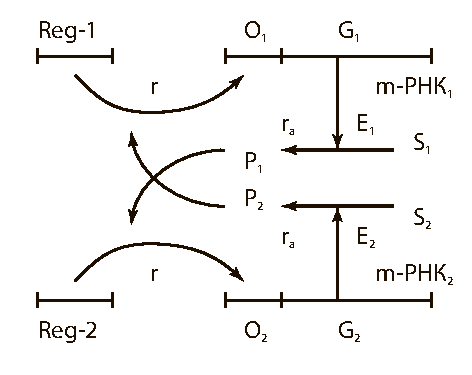
\includegraphics[width=0.5\textwidth]{images/jacob_mono}
    \parbox{0.5\textwidth}{\caption{Схема взаимной регуляции двух 
    систем синтеза фермента}}
\end{wrapfigure}

Рассмотрим модель синтеза фермента \( E \) и катализируемого им продукта 
\( P \). Уравнения запишутся в виде:
\[
    \left\{ \begin{array}{ll}
        \cfrac{dE}{dt} = \cfrac{1}{\tau_E}I - \cfrac{1}{\tau_2}E \\
        \cfrac{dP}{dt} = E\cfrac{k_{+2}S}{K_S + S} - qP \\
        \cfrac{dI}{dt} = Q(r) - \cfrac{1}{\tau_1}I
    \end{array} \right. \eqno{1}
\]
где \( \tau_E \) -- время синтеза молекулы фермента \( E \). Член 
\( E/\tau_2 \) описывает распад фермента за счёт протеолиза, член
\( k_{+2}ES / (K_S + S) \) -- синтез продукта \( P \) из субстрата \( S \) 
с участием фермента \( E \), член \( qP \) -- отток продукта \( P \).

Последнее уравнение описывает синтез m-РНК. Тогда согласно уравнению 
полученного при синтезе m-РНК:
\[ 
    \frac{dI}{dt} = \frac{a_2 a_3}{\tau_0 a_2 a_3 + f(r) + a_3} -
    \frac{1}{\tau_1}I 
\] 

и \( f(r) = k_0 R^m \) скорость синтеза будет:
\[
    Q(r) = \frac{a_2 a_3}{\tau_0 a_2 a_3 + a_3 + k_0 R^m}
\]

В стационарных условиях
\[
    \bar{E} = \frac{\tau_2}{\tau_E}\bar{I};\quad
    \bar{P} = \frac{k_{+2}S}{q(K_S + S)\bar{E}};\quad
    \bar{I} = Q\tau_1
\]

введя обозначения
\[
    x = \frac{E}{\bar{E}};\quad
    y = \frac{P}{\bar{P}};\quad
    z = \frac{I}{\bar{I}};\quad
    t'' = tq
\]

перепишем систему \( (1) \) в виде:
\[
    \left\{ \begin{array}{ll}
        \cfrac{dx}{dt''} = \cfrac{1}{\tau_2 q}\left( z - x \right) \\
        \cfrac{dy}{dt''} = x - y \\
        \cfrac{dz}{dt''} = \cfrac{1}{\tau_1 q}\left( 1 - z \right)
    \end{array} \right. \eqno{2}
\]

Величины \( (\tau_2 q)^{-1} \) и \( (\tau_1 q)^{-1} \) можно считать 
достаточно большими, а первое и третье уравнение -- присоединенными, и 
используя теорему Тихонова приходим к простой модели из одного уравнения:
\[
    \frac{dy}{dt''} = 1 - y
\]

Возвращаясь к прежним обозначениям:
\[
    \frac{dP}{dt} = \frac{k_{+2}S}{K_S + S}\frac{\tau_1\tau_2}{\tau_E}
        \frac{a_2 a_3}{\tau_0 a_2 a_3 + a_3 + k_0 R^m} - qP \eqno{3}
\]

В случае когда \( \tau_2 q \sim 1 \) оставляем два уравнения:
\[
    \left\{ \begin{array}{ll}
        \cfrac{dx}{dt''} = \cfrac{1}{\tau_2 q}\left( 1 - x \right) \\
        \cfrac{dy}{dt''} = x - y
    \end{array} \right. \eqno{4}
\]

или в размерном виде:
\[
    \left\{ \begin{array}{ll}
        \cfrac{dE}{dt} = \cfrac{\tau_1 a_2 a_3}
            {\tau_E\left( \tau_0 a_2 a_3 + a_3 + k_o R^m \right)}
            - \cfrac{1}{\tau_2}E \\
        \cfrac{dP}{dt} = \cfrac{k_{+2}S}{K_S + S} E - qP
    \end{array} \right. \eqno{5}
\]

\section{Триггерная схема Жакоба-Моно}

Модели описываемые уравнениями \( [3] \) и \( [5] \) не являются 
замкнутыми, поскольку не указано, как связаны концентрация активного 
репрессора \( r_a \) и субстрата \( S \) с концентрацией продукта \( P \). 
Кроме того, они описывают поведение одного гена, в то время важно учесть 
влияние работы одного гена на другой. В этом случае величины \( P \) и 
\( S \) могут быть связаны с продуктами деятельности другого гена. В 
качестве простейшего варианта Жакоб и Моно предложили триггерную схему. 
В ней корепрессором первой системы является продукт второй системы 
\( P_2 \) и корепрессором второй -- \( P_1 \).

Рассмотрим случай, когда концентрация субстратов \( S_1 \) и \( S_2 \) 
постоянны. Модель должна состоять из уравнений, описывающих синтез 
\( P_1 \) и \( P_2 \); при этом согласно схеме положим:
\[
    R_1 \equiv P_2;\quad R_2 \equiv P_1
\]

Принимая, что синтез продуктов описывается уравнением \( [3] \), запишем 
модель в виде:
\[
    \left\{ \begin{array}{ll}
        \cfrac{dP_1}{dt} = \cfrac{A_1}{B_1 + P_2^m} - q P_1 \\
        \cfrac{dP_2}{dt} = \cfrac{A_2}{B_2 + P_1^m} - q P_2
    \end{array} \right. \eqno{6}
\]

Здесь величины \( A \) и \( B \) выражаются через параметры своих систем 
следующим образом:
\[
    A = \frac{k_{+2} a_2 a_3 \tau_1 \tau_2 S}{(K_S + S) k_0 \tau_E};\quad 
    B = \frac{\tau_0 a_2 a_3 + a_3}{ k_0 }
\]

Введём безразмерные переменные:
\[
    x_1 = \frac{P_1}{B^{1/m}_1};\quad
    x_2 = \frac{P_2}{B^{1/m}_2};\quad
    L_1 = \frac{A_1}{q B_1};\quad
    L_2 = \frac{A_2}{q B_2};\quad
    t' = qt
\]

опустив штрих у времени, перепишем систему \( [6] \) в виде:
\[
    \left\{ \begin{array}{ll}
        \cfrac{dx_1}{dt} = \left[ \cfrac{1}{B_1^{1/m}} \right]
        \cdot\cfrac{L_1}{1+\gamma x_2^m} - x_1 \\
        \cfrac{dx_2}{dt} = \left[ \cfrac{1}{B_2^{1/m}} \right]
        \cdot\cfrac{L_2}{1+\gamma^{-1} x_1^m} - x_2
    \end{array} \right. \eqno{7}
\]

где \( \gamma = B_2 / B_1 \).
\[
    \left\{ \begin{array}{ll}
        \cfrac{dx_1}{dt} = \cfrac{L_1}{1+\gamma x_2^m} - x_1 \\
        \cfrac{dx_2}{dt} = \cfrac{L_2}{1+\gamma^{-1} x_1^m} - x_2  
    \end{array} \right. \eqno{8}
\]

\section{Исследование триггерной системы}

Рассмотрим поведение системы при \( m = 2 \). Тогда уравнение \( [8] \) 
перепишем в виде
\[
    \left\{ \begin{array}{ll}
        \cfrac{dx_1}{dt} = \cfrac{L_1}{1+\gamma x_2^2} - x_1 \\
        \cfrac{dx_2}{dt} = \cfrac{L_2}{1+\gamma^{-1} x_1^2} - x_2  
    \end{array} \right. \eqno{9}
\]

Решая систему приближенным методом, будём варьировать параметры 
\( L_1, L_2 \) и \( \gamma \) системы при различных начальных условиях. 

%\begin{figure}[!]
%    \center
%    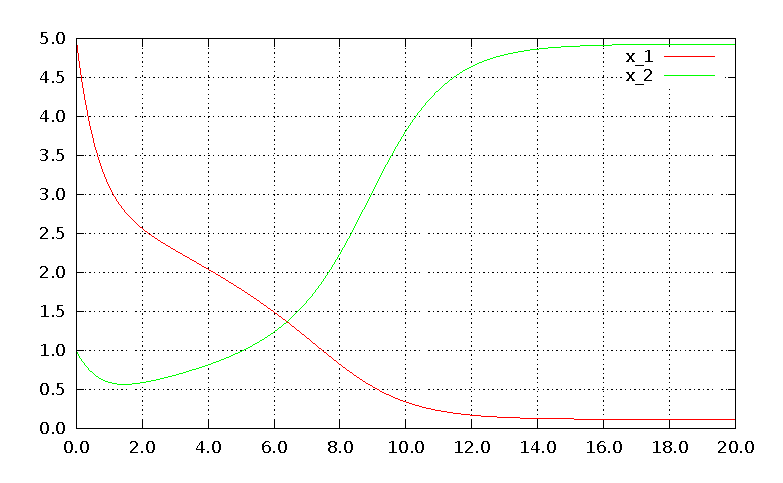
\includegraphics[width=0.8\textwidth]{images/graph1}
%    \parbox{\textwidth}{\caption{Изменение концентрации продукта с течением времени}}
%    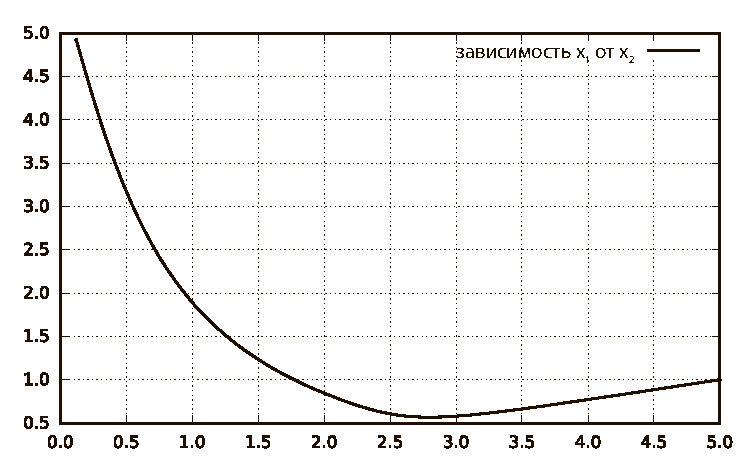
\includegraphics[width=0.8\textwidth]{images/graph2}
%    \parbox{\textwidth}{\caption{Зависимость \( x_1 \) от \( x_2 \)}}
%\end{figure}

%Полученные графики построены при значения \( x_{10} = 5 \), \( x_{20} = 1 \), 
%\( L_1 = 3 \) и \( L_2 = 5 \). При большых разницах в начальных значениях
%концентраций -- система быстро переходит из одного состояния в другое. 

\newpage

\section{Список использованной литературы}
    \begin{enumerate}
        \item Ризниченко, Г.Ю. Лекции по математическим моделям в 
            биологии. Ч.1. -- Ижевск: НИЦ
            <<Регулярная и хаотическая динамика>>, 2002, 232 с.
        \item Романовский, Ю.М. Математическое моделирование в биофизике
            -- Москва: <<Наука>>, 1975, 335 с.
    \end{enumerate}